\documentclass[a4paper, 11pt]{article}

\usepackage[utf8]{inputenc}
\usepackage[left=2cm,text={17cm, 24cm},top=3cm]{geometry}
\usepackage[unicode, colorlinks]{hyperref}
\usepackage[czech]{babel}
\usepackage{graphicx}
\usepackage{multirow}
\usepackage{float}
\usepackage{pdflscape}
\usepackage{caption}
\usepackage{amssymb}
\usepackage{amsmath}
\usepackage{mathtools}
\usepackage{fancyhdr}
\usepackage{listings}
\usepackage{color}
\usepackage[dvipsnames,svgnames,table]{xcolor}

\lstset{
    basicstyle=\small\ttfamily,
    columns=flexible,
    breaklines=true
}
\lstset{literate=%
    {á}{{\'a}}1
    {í}{{\'i}}1
}
\lstset{extendedchars=\true}
\lstset{inputencoding=ansinew}

\renewcommand{\arraystretch}{1.5}


\fancyhf{}
\fancyhead[L]{VUT FIT IVS 2016/2017}
\fancyhead[C]{/dej/uran/dom}
\fancyhead[R]{Uživatelská dokumentace}
\fancyfoot[C]{\thepage}

\begin{document}

\thispagestyle{empty}

\begin{figure}[H]
    \centering
    
\includegraphics[width=.5\textwidth]{logo.png}
    \vspace{32pt}

    {\Huge{\textbf{Uživatelská dokumentace}}}\\
    \vspace{20pt}
    \texttt{/dej/uran/dom}\\
    \textit{xkolar71} Josef Kolář\\
    \textit{xnguye16} Son Hai Nguyen\\
    \textit{xomach00} Martin Omacht\\
    \textit{xnavra61} Robert Navrátil
\end{figure}

\hypersetup{
    colorlinks=true,
    linktoc=all
}

{\hypersetup{linkcolor=black}
\tableofcontents
}

\hypersetup{urlcolor = {blue}}

\newpage

\pagestyle{fancy}

\section{Úvod}\label{uvod}

Calculator je grafická kalkulačka jako školní projekt do předmětu IVS na FIT VUT v letním semestru školního roku 2016/2017. Kalkulačka nabízí plnohodnotné matematické funkce, systém proměnných (včetně jejich zavislostí) i skrytý easter egg. Jádro aplikace, které je naimplementováno v programovacím jazyce \\v~\href{https://www.python.org/}{Python}, je kompletně pokryto jednotkovými testy. Nad tímto jádrem je postavena grafická vrstva pomocí frameworku \href{https://www.qt.io/}{Qt}.

\section{Instalace}
Aplikaci je možné nainstalovat jako:
\begin{enumerate}
    \item instalační balíček operačního systému Debian, který je dostupný na adrese z~\href{https://github.com/thejoeejoee/IVS-VUT-BIT-2016-2017/releases/latest}{posledního vydání} aplikace nebo v \textbf{odevzdaném distribučním balíku ve složce \texttt{install/}}- instalace pak probíhá následovně: \\
    \begin{lstlisting}
    // instalace závislostí
    # apt install python3-all python3-pip python3-opengl
    // instalace balíku
    # dpkg -i python3-calculator_XXXX.deb
    \end{lstlisting}
    \item instalace jako standardní balíček jazyka Python pomocí skriptu \texttt{setup.py} v kořenu repozitáře aplikace:
    \begin{lstlisting}[breaklines]
    $ git clone https://github.com/thejoeejoee/IVS-VUT-BIT-2016-2017.git calculator
    $ cd calculator
    # python3 setup.py install
    \end{lstlisting}
\end{enumerate}

V obou případech je do systému nainstalován grafický spouštěč. Ten hledejte
v menu vašeho systému. Také jsou nainstalovány spustitelné skripty
\texttt{calculator}     a \texttt{calculator-console}, z nichž první spouští
grafické rozhraní aplikace, druhý pouze konzolovou verzi kalkulačky.

\section{Odinstalace}

Zde záleží, kterým způsobem byla kalkulačka nainstalována.
\begin{enumerate}
    \item balíček operačního systému Debian, pak pomocí standardního balíčkovacího systému \texttt{apt}:
    \begin{lstlisting}
    # apt remove python3-calculator
    \end{lstlisting}
    \item Python balíček (požadována Python utilita \texttt{pip3} pro správu balíčků):
    \begin{lstlisting}
    # pip3 uninstall calculator
    \end{lstlisting}
\end{enumerate}

\section{Návod}

V této kapitole bude popsána práce v \textbf{Calculator}u, jeho funkce a užitečné
vlastnosti, a dále také základní panely pro práci.

\subsection{Matematické funkce}

Ve všech funkcích lze použít klasické operátory (+, -, *, /) a i jiné
funkce.
\begin{table}[H]
    \catcode`\-=12
    \centering
    \begin{tabular}{|p{3cm}|p{6.25cm}|p{6.25cm}|}
        \hline
        \multicolumn{1}{|c|}{\bfseries Zápis}   & \multicolumn{1}{c|}{\bfseries Význam}    & \multicolumn{1}{c|}{\bfseries Poznámka} \\ \cline{1-3}
        $ \text{abs}(x)$  & \multirow{2}{*}{\begin{minipage}{6.25cm}Funkce pro výpočet absolutní hodnoty zadaného čísla.\end{minipage}} & \multirow{2}{*}{}  \\ \cline{1-1}
        $|x|$     &           &           \\ \cline{1-3}
        $\text{fact}(x)$   & \multirow{2}{*}{Výpočet faktorialu zadaného čísla.}   & \multirow{2}{*}{\begin{minipage}{6.25cm}Hodnota faktorialu je kvůli prudkému nárůstu omezena.\end{minipage}} \\ \cline{1-1}
        $x!$    &   &   \\ \cline{1-3}
        \multirow{2}{*}{$\text{ln}(x)$}  & \multirow{2}{*}{\begin{minipage}{6.25cm}Funkce počítá přirozený logaritmus čísla $x$.\end{minipage}} & Přirozený logaritmus má základ $e$ (Eulerovo číslo). \\ \cline{1-3}
        \multirow{2}{*}{$\log(x, y)$}   & \multirow{2}{*}{\begin{minipage}{6.25cm}Výpočet obecného logaritmu se zadaným základem.\end{minipage}} & x = logaritmované číslo \\
            &   & y = základ logaritmu \\ \cline{1-3}
        $\text{pow}(x,y)$   & \multirow{2}{*}{Funkce pro výpočet mocniny.}  & x = mocněné číslo (mocněnec) \\ \cline{1-1}
        $x**y$  &   & y = mocnitel \\ \cline{1-3}
        $\text{rand}()$  & Funkce, která vygeneruje náhodné reálné číslo v rozsahu $\langle 0, 1 \rangle$. & Funkce nemá žádný parametr. \\ \cline{1-3}
        \multirow{2}{*}{$\text{root}(x, y)$} & \multirow{2}{*}{Funkce pro výpočet obecné odmocniny.}  & x = odmocňované číslo \\
            &   & y = y-tá odmocnina \\ \cline{1-3}
        $\text{sqrt}(x)$    & Funkce pro výpočet 2. odmocniny. & \\ \cline{1-3}
    \end{tabular}
\end{table}

\subsection{Komponenty grafického rozhraní}

\subsubsection{Číselné soustavy}

Pokud je výsledek \emph{celočíselný}, tak bude výsledek převeden a
zobrazen ve 4 číselných soustavách (dvojkové, osmičkové, desítkové,
šestnáctkové). Velký výsledek, který se nevyobrazí v okně celý, je možné
zobrazit posunutím výsledku v příslušné číselné soustavě (stačí podržet levé tlačítko myši, a potom posunout požadovaným směrem).

\begin{figure}[H]
    \centering
    \frame{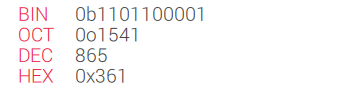
\includegraphics[scale=0.7]{system2.png}}
    \caption{Číselné soustavy s převedeným číslem}
\end{figure}

\subsubsection{Funkce a zápisové okno}

Jednou z hlavních částí je panel s funkcemi a k němu navazující okno s
výrazem k výpočtu.

\begin{figure}[H]
    \centering
    \frame{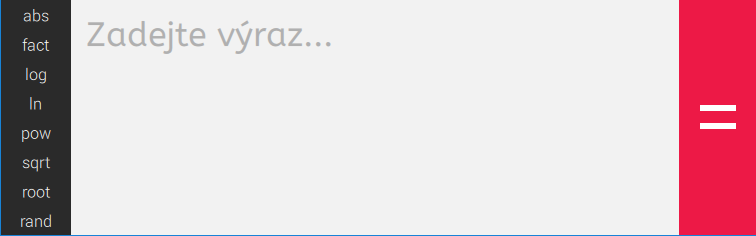
\includegraphics[scale=0.75]{func2.png}}
    \caption{Panel s funkcemi a výrazovým oknem}
\end{figure}

\subsubsection{Proměnné}

\textbf{Calculator} umí také používat proměnné, takže si můžete uložit výpočty do
proměnných a dále je používat. Panel proměnných obsahuje také posuvník,
pokud je proměnných příliš mnoho. Je vhodné poznamenat, že u názvů proměnných je nutno respektovat velikost písmen.

\begin{figure}[H]
    \centering
    \frame{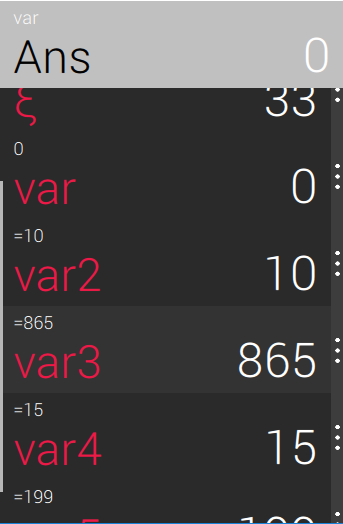
\includegraphics[scale=0.5]{variable.png}}
    \caption{Panel proměnných}
\end{figure}

Pro identifikátor můžete použít jakýkoliv Unicode znak, který neodporuje
běžným matematickým konstrukcím a znakům jako například uvozovky, operátory apod.

\subsection{Práce s kalkulačkou}

\subsubsection {Prace přes gracfické uživatelské rozhraní}

\textbf{Calculator} obsahuje funkce, které Vám mohou zrychlit práci.
Jednou z těchto funkcí je doplňování kódu klávesovou zkratkou
\texttt{ ctrl+space }. Toto menu obsahuje vytvořené proměnné i vestavěné funkce.

\begin{figure}[H]
    \centering
    \frame{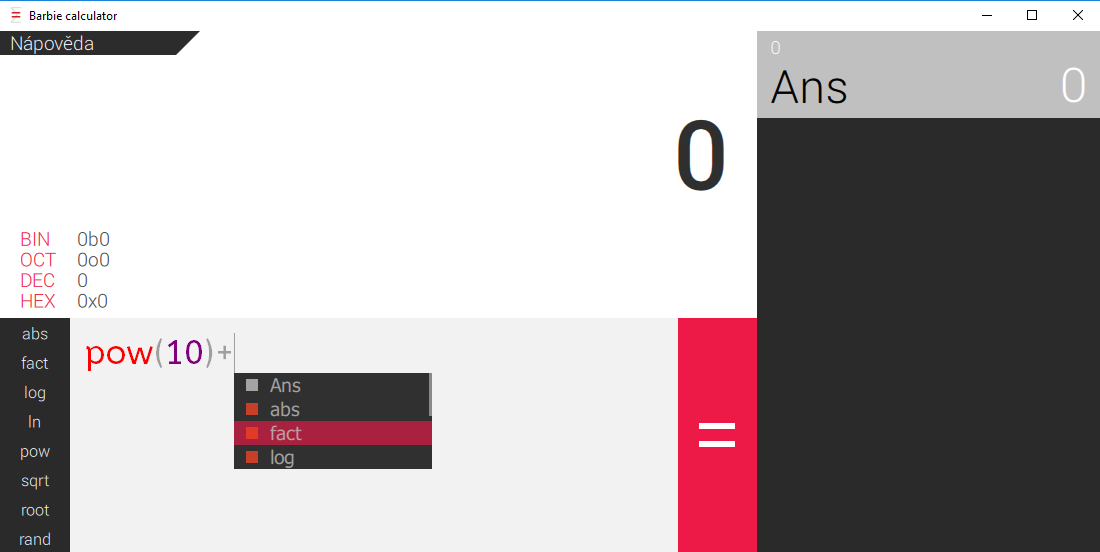
\includegraphics[scale=0.6]{complete.png}}
    \caption{Doplňování kódu}
\end{figure}

Dále také rozšíření závorek a výrazů do funkcí. Výraz, který chcete
vložit do funkce nebo závorek označíte a kliknete na funkci nebo
napíšete levou závorku \texttt{(}.

\begin{figure}[H]
    \centering
    \frame{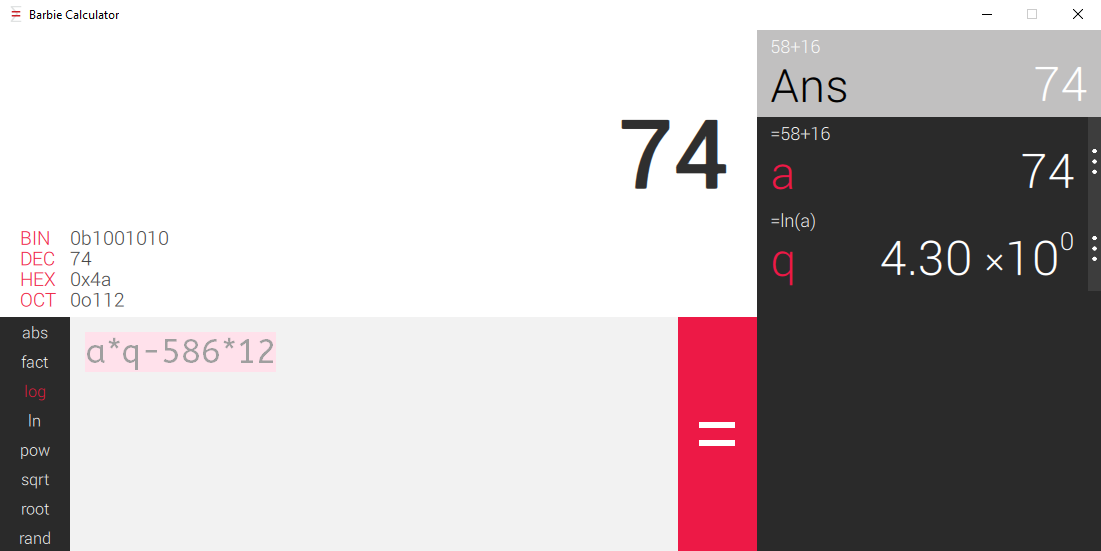
\includegraphics[scale=0.6]{enfunc1.png}}
    \caption{Výraz před použitím funkce}
\end{figure}

\begin{figure}[H]
    \centering
    \frame{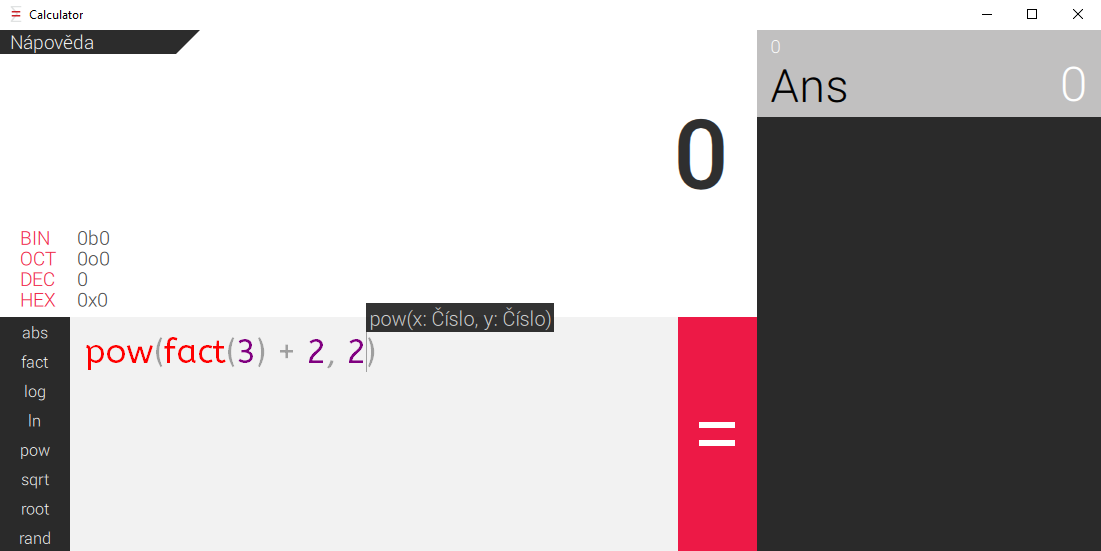
\includegraphics[scale=0.6]{enfunc2.png}}
    \caption{Výraz po použití funkce}
\end{figure}

Také je třeba zmínit práci s proměnnými. Proměnné lze mazat v menu (tři
tečky) pomocí ikony koše, a také nastavit na \texttt{1} nebo \texttt{0}.
Pravým kliknutím myši se Vám do výrazového okna zkopíruje hodnota
proměnné a levým kliknutím myši její identifikátor.

\begin{figure}[H]
    \centering
    \frame{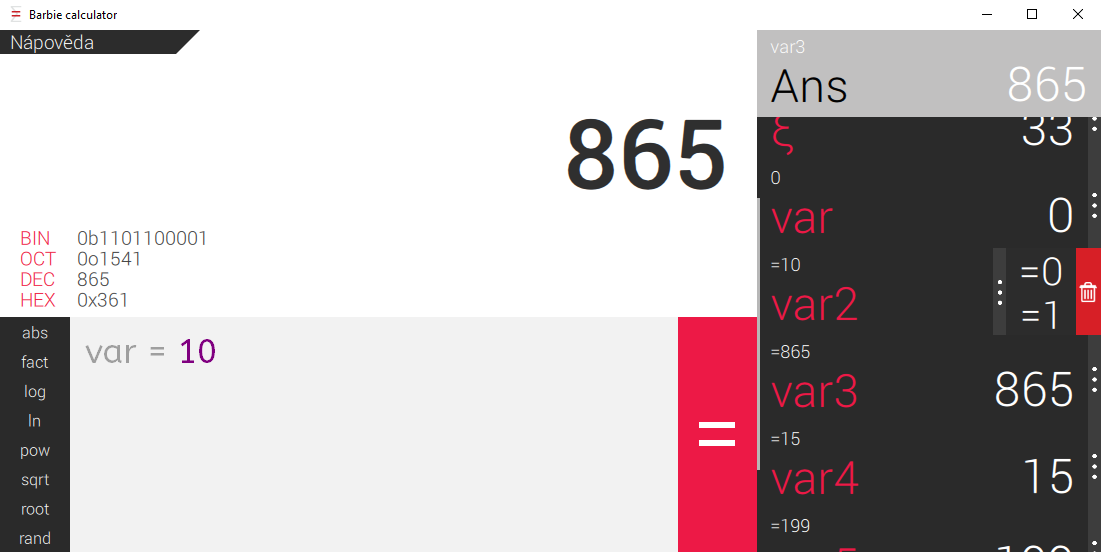
\includegraphics[scale=0.6]{many_vars.png}}
    \caption{Mnoho proměnných a jejich nastavení}
\end{figure}

\noindent
\textbf{Calculator} má také vestavěnou nápovědu funkcí.

\begin{figure}[H]
    \centering
    \frame{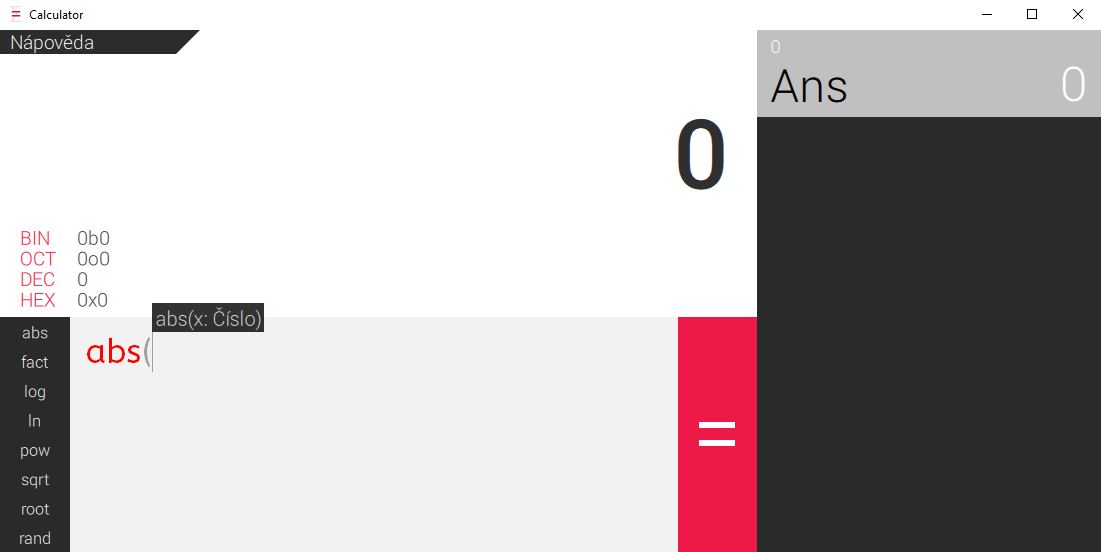
\includegraphics[scale=0.6]{help_func.png}}
    \caption{Nápověda u funkce}
\end{figure}

\noindent
Poslední vlastností je zápis v různých soustavách, který se provádí pomocí
prefixů:
\begin{itemize}
    \item \texttt{0b{[}číslo{]}} pro dvojkovou soustavu
    \item \texttt{0o{[}number{]}} pro osmičkovou soustavu
    \item \texttt{0x{[}number{]}} pro šestnáctkovou soustavu
\end{itemize}

\begin{figure}[H]
    \centering
    \frame{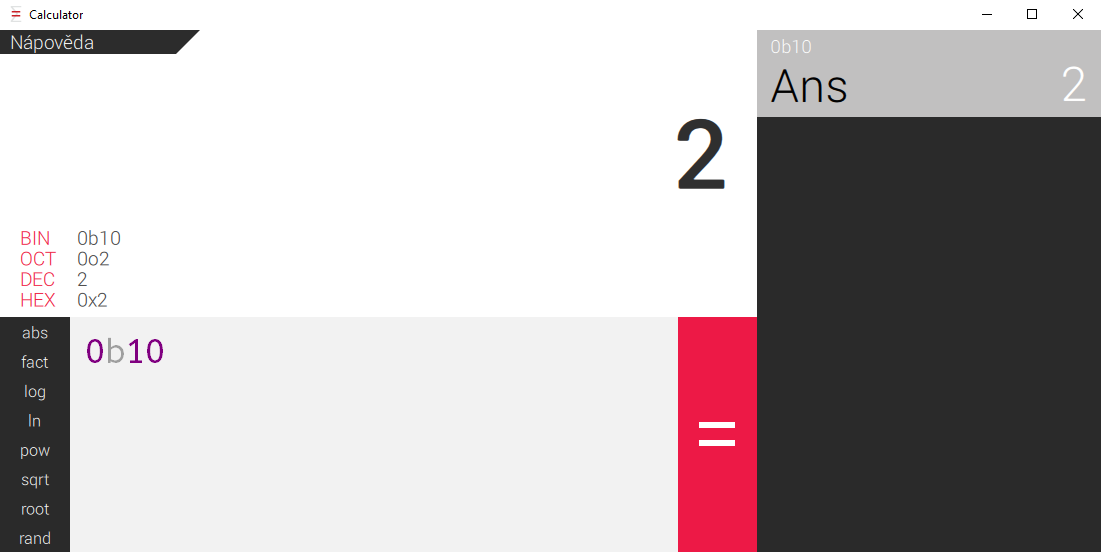
\includegraphics[scale=0.6]{binary_value.png}}
    \caption{Zápis ve dvojkové soustavě}
\end{figure}

\subsubsection{Práce přes rozhraní příkazové řádky}
\texttt{Calculator} poskytuje také rozhraní příkazové řádky, které se spouští příkazem\texttt{ calculator-console}.
V tomto rozhraní můžete zadávat stejné matematické výrazy jako v grafickém rozhraní kalkulačky. Výrazy se dají oddělit středníkem (\texttt{;}), v takovém případě se výrazy vyhodnotí postupně za sebou. Po zadání výrazu kalkulačka vypíše výsledek (v případě přiřazování do prměnné nevypíše nic).

Pro výpis proměnných je k dispozici příkaz\texttt{ \%print [<var>]}, který akceptuje jako volitelný parametr jméno proměnné. Pokud je parametr specifikován, vypíše se pouze daná proměnná. Při zavolání bez perametru se vypíší všechny proměnné.
\vspace{0.5cm}

\noindent
Příklady použití:

\noindent\texttt{\$ calculator-console} \\
\texttt{>>> x = -4} \\
\texttt{>>> x**3 - sqrt(|x|) + 12} \\
\texttt{=== -54.0} \\[0.5cm]
\texttt{>>> x = 8} \\
\texttt{>>> \%print} \\
\texttt{\-\ \ Ans === 521.1715728752538 \ (x**3 - sqrt(|x|) + 12)} \\
\texttt{\-\ \ \ \ x === 8 \ (x = 8)} \\[0.5cm]
\texttt{>>> \%print x} \\
\texttt{\-\ \ \ \ x === 8 \ (x = 8)} \\[0.5cm]

\subsection{Easter egg}

\begin{center}

\bfseries
\fontsize{96pt}{32pt}
    {\color[RGB]{255,125,125} N}%
    {\color[RGB]{255,249,121} Y}%
    {\color[RGB]{111,255,106} A}%
    {\color[RGB]{255,145,250} N}%
\- = 42
\end{center}

\end{document}
